\documentclass[cal1spr16Lectures.tex]{subfiles}

\begin{document}

\section[]{}

% % %
\subsection[5.1 Approximating Area Under Curves]{\S 5.1 Approximating Area Under Curves}
% % %

% % %
\begin{frame}{\S 5.1 Approximating Area Under Curves}\small
In the previous two chapters, we have come to see the derivative of a function associated with the rate of change of a function as well as the slope of the tangent line to the curve.
\vspace{1pc}

In the first section of Chapter 5, we now examine the meaning of the integral.
\begin{que}
If we know the velocity function of a particular object, what does that tell us about its position function?
\end{que}
\end{frame}

% % %
\begin{frame}\small
\begin{ex} 
Suppose you ride your bike at a constant velocity of 8 miles per hour for 1.5 hours.
\begin{itemize}
\item[(a)] What is the velocity function that models this scenario?
\item[(b)] What does the graph of the velocity function look like?
\item[(c)] What is the position function for this scenario?
\item[(d)] Where is the displacement (i.e., the distance you've traveled) represented when looking at the graph of the velocity function?
\end{itemize}
\end{ex}
\end{frame}

% % %
\begin{frame}\small
In the previous example, the velocity was constant.  In most cases, this is not accurate (or possible).  How could we find displacement when the velocity is changing over an interval?
\vspace{1pc}

One strategy is to divide the time interval into a particular number of subintervals and approximate the velocity on each subinterval with a constant velocity.  Then for each subinterval, the displacement can be evaluate and summed.
\vspace{1pc}

{\bf Note:}  This provides us with only an approximation, but with a larger number of subintervals, the approximation becomes more accurate.
\end{frame}

% % %
\begin{frame}\footnotesize
\begin{ex} 
Suppose the velocity of an object moving along a line is given by $v(t)=\sqrt{10t}$ on the interval $1 \le t \le 7$.  Divide the time interval into $n=3$ subintervals, assuming the object moves at a constant velocity equal to the value of $v$ evaluated at the midpoint of the subinterval.  Estimate the displacement of the object on $[1,7]$.  Repeat for $n=6$ subintervals. 
\vspace{-0.5pc}
\begin{center}
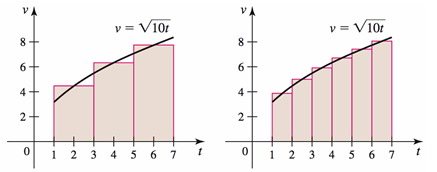
\includegraphics[scale=0.75]{pictures/Ch5Sect1_Exer10}
\end{center}
\end{ex}
\end{frame}

% % %
\subsubsection{Riemann Sums}
% % %

% % %
\begin{frame}{\small Riemann Sums}\footnotesize
The more subintervals you divide your time interval into, the more accurate your approximation of displacement will be.% (see Example 1 on pp.\ 307--308).
We now examine a method for approximating areas under curves.

\vspace{1pc}
Consider a function $f$ over the interval $[a,b]$.  Divide $[a,b]$ into $n$ subintervals of equal length:
\[[x_0,x_1], [x_1,x_2], \dots, [x_{n-1},x_n]\]
with $x_0=a$ and $x_n=b$.  The length of each subinterval is denoted
\[\Delta x = \frac{b-a}{n}.\]
\end{frame}

% % %
\begin{frame}\footnotesize
In each subinterval $[x_{k-1}, x_k]$ (where $k$ is any number from $1$ to $n$), we can choose any point $\overline{x}_k$ (note $\overline{x}_k$ might be different, depending on which $k$), and create a rectangle with a height of $f(\overline{x}_k)$.

\vspace{1pc}
The area of the rectangle is ``base times height", written $f(\overline{x}_k)\Delta x$, since the base is the length of the subinterval.

\vspace{1pc}
Doing this for each subinterval, and then summing each rectangle's area, produces an approximation of the overall area.  This approximation is called a {\bf Riemann sum}
\[R=f(\overline{x}_1)\Delta x + f(\overline{x}_2)\Delta x + \cdots + f(\overline{x}_n)\Delta x.\]
The symbol ``$k$" is what's known as an {\bf indexing variable}.  We let $k$ vary from $1$ to $n$, and we always have $x_{k-1}\leq \overline x_k\leq x_k$.  
\end{frame}

% % %
\begin{frame}{}{}\footnotesize
{\bf Note:} We usually choose $\overline{x}_k$ so that it is consistent across all the subintervals.  
\begin{dfn}
Suppose
\[
R=f(\overline{x}_1)\Delta x + f(\overline{x}_2)\Delta x + \cdots + f(\overline{x}_n)\Delta x
\]
is a Riemann sum.  Then:
\begin{itemize}
\item[1.] $R$ is a {\bf left Riemann sum} when we choose $\overline x_k=x_{k-1}$ for each $k$ (so $\overline x_k$ is the left endpoint of the subinterval).  
\item[2.] $R$ is a {\bf right Riemann sum} when we choose $\overline x_k=x_k$ for each $k$ (so $\overline x_k$ is the right endpoint of the subinterval).
\item[3.] $R$ is a {\bf midpoint Riemann sum} when we take $\overline x_k$ to be the midpoint between $x_{k-1}$ and $x_k$, for each $k$.  
\end{itemize}
\end{dfn}
(See pages 337-339 for picture of these.)
\end{frame}

% % %
\begin{frame}\footnotesize
\begin{ex}
Calculate the left Riemann sum for the function $f(x)=x^2-1$ on the interval $[2,4]$ when $n=4$.
\begin{itemize}
\item[A.] 13.75
\item[B.] 19.75
\item[C.] 27.5
\item[D.] 55
\end{itemize}
\end{ex}
\begin{exe}
Compute the left, right, and midpoint Riemann sums for the function $f(x)=2x^3$ on the interval $[0,8]$ with $n=4$.
\end{exe}
\end{frame}

% % %
\subsubsection{Sigma Notation}
% % %

% % %
\begin{frame}{\small Sigma Notation}\footnotesize
Riemann sums become more accurate when we make $n$ (the number of rectangles) bigger, but obviously writing it all down is no fun!  Sigma notation gives a shorthand.  Here is how sigma notation works, through an example: 
\begin{ex} 
$\sum_{n=1}^5 n^2$ is the sum all integer values from the lowest limit ($n=1$) to the highest limit ($n=5$) in the summand $n^2$ (in this case $n$ is the indexing variable).  
\[\sum_{n=1}^5 \alert n^2 = \alert 1^2+\alert 2^2+\alert 3^2+\alert 4^2+\alert 5^2=55.\] 
\end{ex}
\end{frame}

% % %
\begin{frame}\small
\begin{ex} 
Evaluate $\sum_{k=0}^3 (2k-1)$. 
\end{ex}
\footnotesize
{\bf Solution:} In this example, $k$ is the indexing variable.  It starts at $0$ and goes to $3$, which means we write down the expression in the parentheses for each of the integers from $0$ to $3$, then add the results together:
\begin{align*}
\sum_{k=0}^3(2\alert k-1) &= (2(\alert 0)-1)+(2(\alert 1)-1)+(2(\alert 2)-1)+(2(\alert 3)-1) \\
	&= -1+1+3+5 = 8.
\end{align*}
\end{frame}

% % %
\subsubsection{$\Sigma$-Shortcuts}
% % %

% % %
\begin{frame}{\small $\Sigma$-Shortcuts}\footnotesize
($n$ is always a positive integer)
\vspace{-1pc}
\begin{align*}
\sum_{k=1}^n c & = cn \text{ (where $c$ is a constant)} \\%[0.25pc]
\sum_{k=1}^n k &= \dfrac{n(n+1)}{2} \\%[0.25pc]
\sum_{k=1}^n k^2 &= \dfrac{n(n+1)(2n+1)}{6} \\%[0.25pc]
\sum_{k=1}^n k^3 &= \dfrac{n^2(n+1)^2}{4}
\end{align*}
\vspace{-1.5pc}
\begin{que}
What is the indexing variable in these formulas?
\end{que}
\end{frame}

% % %
\subsubsection{Riemann Sums Using Sigma Notation}
% % %

% % %
\begin{frame}{\small Riemann Sums Using Sigma Notation}\footnotesize
Suppose $f$ is defined on a closed interval $[a,b]$ which is divided into $n$ subintervals of equal length $\Delta x$.  As before, $\overline{x}_k$ denotes a point in the $k$th subinterval $[x_{k-1},x_k]$, for $k=1,2,\dots,n$.  Recall that $x_0=a$ and $x_n=b$. 

\vspace{1pc}
Here is how we can write the Riemann sum in a much more compact form:
\vspace{-1pc}
\[
R = f(\overline{x}_1)\Delta x + f(\overline{x}_2)\Delta x + \cdots + f(\overline{x}_n)\Delta x 
 = \alert{\sum_{k=1}^n f(\overline{x}_k) \Delta x}.
\]
\end{frame}

% % %
\begin{frame}
With sigma-notation we can even derive explicit formulas for the basic Riemann sums (the expression in \alert{red} is $\overline x_k$ for each case:

\begin{itemize}
\item[1.] $\displaystyle\sum_{k=1}^n f(\alert{a+(k-1)\Delta x}) \Delta x=$ left Riemann sum
\item[2.] $\displaystyle\sum_{k=1}^n f(\alert{a+k\Delta x}) \Delta x=$  right Riemann sum
\item[3.] $\displaystyle\sum_{k=1}^n$\hspace{-1pt} $f(\alert{a+\left(k-\frac{1}{2}\right)\Delta x}) \Delta x=$ midpoint Riemann sum
\end{itemize}
\end{frame}

\begin{frame}\small
\begin{exe} 
\begin{itemize}
\item[(a)] Use sigma notation to write the left, right, and midpoint Riemann sums for the function $f(x)=x^2$ on the interval $[1,5]$ given that $n=4$.
\item[(b)] Based on these approximations, estimate the area bounded by the graph of $f(x)$ over $[1,5]$.
\end{itemize}
\end{exe}
{\bf Suggestion:} As $n$ gets very big, Riemann sums, along with the $\Sigma$-shortcuts plus algebra, often make the problem way more manageable. 
\end{frame}

% % %
\subsubsection{Book Problems}
% % %

% % %
\begin{frame}
\begin{block}{5.1 Book Problems}
9-37
\end{block}
\end{frame}

\end{document}